\documentclass[11pt]{article}
\usepackage[margin=0.9in]{geometry}
\usepackage{amsmath,amssymb,graphicx,booktabs,natbib}
\usepackage[colorlinks=true,allcolors=blue]{hyperref}
\setlength{\emergencystretch}{1em}
\hypersetup{pdftitle={When History Can Replace Action Chunking},pdfauthor={Nihar Ballamudi and Kyle Horton}}
\newcommand{\norm}[1]{\left\lVert#1\right\rVert}
\newcommand{\spr}{\operatorname{spr}}
\begin{document}
\begin{center}
{\Large\bfseries When History Can Replace Action Chunking}\\[5pt]
Nihar Ballamudi and Kyle Horton --- University of Pennsylvania
\end{center}
\noindent\textbf{Abstract.}
We connect observability, incremental chunk stability, and recovery experiments on the linear challenging pair. Sufficient history permits exact noiseless one-step imitation, but restricted demonstrations need not identify that policy. We give a conditional certificate for general learners and an explicit small-gain certificate for the ridge learner. In the current noiseless sweep, history eight requires execution length eight under the chosen criterion, whereas history sixteen permits execution length one. These results separate state information from feedback selection; they do not establish universal monotonicity of tracking loss.

\section{History supplies information; learning selects feedback}
Consider $x_{t+1}=Ax_t+Bu_t$, $y_t=Cx_t$, and expert $u_t^*=Kx_t$, with $F=A+BK$. Restricted demonstrations can conceal recovery behavior even for stable plants and experts \citep{simchowitz2025}; commitment can suppress destabilizing learned feedback \citep{zhang2025}. We ask whether history reduces the need for that commitment.

The learner observes $z_t^{(r)}=\operatorname{col}(y_{t-r+1:t},u_{t-r+1:t-1})$. Context $r$ counts observations, prediction horizon $H$ counts predicted actions, and execution $\ell\le H$ counts actions committed before replanning. Let $h=\min\{r:\operatorname{rank}\mathcal O_r=n\}$, where $\mathcal O_r=\operatorname{col}(C,CA,\ldots,CA^{r-1})$. Reconstruction assumes noiseless measurements, known applied inputs, known dynamics, and a valid initial history.

\noindent\textbf{Proposition 1 (action recovery and execution equivalence).}
An exact current-action policy exists on all noiseless histories iff
\[
\ker\mathcal O_r\subseteq\ker(KA^{r-1}).
\]
For $r\ge h$, state reconstruction is $x_t=R_rz_t$, with
\[
R_r=[A^{r-1}\mathcal O_r^\dagger\quad
\mathcal R_r-A^{r-1}\mathcal O_r^\dagger\mathcal T_r],
\]
where $Y=\mathcal O_rx_{t-r+1}+\mathcal T_rU$ and
$x_t=A^{r-1}x_{t-r+1}+\mathcal R_rU$ define the usual input maps.
The chunk policy $\pi_k^*(z)=KF^kR_rz$ then reproduces the expert for every execution length $1\le\ell\le H$.

\emph{Proof.} Identical histories with identical inputs differ initially by $d\in\ker\mathcal O_r$; their current expert actions differ by $KA^{r-1}d$. Kernel inclusion is necessary and sufficient for action recovery. When $r\ge h$, left inversion and propagation give $R_r$. Applying $KF^kx_b$ produces $x_{b+k}=F^kx_b$ by induction. $\square$

Thus observability removes a representational need for chunking, not a statistical learning difficulty. Noiseless expert histories have rank at most $n$; narrow histories can have rank one. More context can enlarge the set of unidentified coefficients. Under shared process disturbances, one-step tracking obeys $d_{t+1}=Fd_t+Be_t$, where $e_t=\hat\pi(z_t)-Kx_t$. If $\norm{F^k}\le M\beta^k$ and deployment error is at most $\varepsilon$, then
$\limsup_t\norm{d_t}\le M\norm{B}\varepsilon/(1-\beta)$.
Training MSE alone does not supply this deployment bound.

\newpage
\section{Chunk stability and a conditional history tradeoff}
\noindent\textbf{Proposition 2 (Horton's history-based chunk guarantee).}
Let $\norm{z}_{\mathcal Z}$ sum the Euclidean norms of its observation/action blocks. Suppose all admissible trajectory pairs satisfy
\[
\norm{\delta y_{t+k}}\le C_0\rho^k\norm{\delta z_t}_{\mathcal Z}
+C_0\sum_{i<k}\rho^{k-1-i}\norm{\delta u_{t+i}},
\]
with $C_0\ge1$ and $0<\rho<1$. Use the same policy and schedule on both trajectories, $u_{j\ell+k}=\pi_k(z_{j\ell})+v_{j\ell+k}$, with
$\operatorname{Lip}_{\mathcal Z}(\pi_k)\le D\rho^k$. For $0<\alpha<1$, set
\[
\bar\rho=\rho^{1-\alpha},\quad C_r=2rC_0\rho^{-(r-1)},\quad
\bar C=C_0\left(1+\frac{D}{e\alpha\rho\log(1/\rho)}\right).
\]
If $\ell\ge\max(1,r-1)$ and $C_r(1+D\ell/\rho)\rho^{\alpha\ell}\le1$, then
\[
\norm{\delta y_t}\le\bar C\bar\rho^t\norm{\delta z_0}_{\mathcal Z}
+\bar CC_r\sum_{i<t}\bar\rho^{t-1-i}\norm{\delta v_i}.
\]
\emph{Proof sketch.} With $Z_j=\norm{\delta z_{j\ell}}_{\mathcal Z}$ and $V_i=\norm{\delta v_i}$, substitute
$\norm{\delta u_{j\ell+k}}\le D\rho^kZ_j+V_{j\ell+k}$ into the assumed bound. Summing the blocks of the next history gives
\[
Z_{j+1}\le C_r(1+D\ell/\rho)\rho^\ell Z_j
+C_r\sum_{i<\ell}\rho^{\ell-1-i}V_{j\ell+i}.
\]
The first coefficient is at most $\bar\rho^\ell$. Iterate and use
$k\rho^{\alpha k}\le[e\alpha\log(1/\rho)]^{-1}$ within chunks. $\square$

For observable Schur-stable linear plants with $r\ge h$, reconstruction yields the assumed output bound, with suitable constants. This completes the supplied draft's argument, but \emph{does not prove that context shortens execution}: $C_r$ grows with $r$, and $\ell\ge r-1$ cannot certify $r=16,\ell=1$.

\medskip
\noindent\textbf{Proposition 3 (conditional certificate for general learners).}
Choose a norm with $\norm{F}\le a<1$. Suppose an arbitrary deterministic learner satisfies, on every admissible deployment history,
\[
\norm{\hat\pi_{r,j}(z_t)-KF^jx_t}\le\gamma_r q^j\norm{x_t},\qquad 0<q<1.
\]
A sufficient condition for exponential stability is
\[
G(r,\ell):=a^\ell+\gamma_r\sum_{j<\ell}\norm{A^{\ell-1-j}B}q^j<1.
\]
\emph{Proof.} Writing the prediction residual as $e_j$, unrolling gives
$x_{t+\ell}=F^\ell x_t+\sum_{j<\ell}A^{\ell-1-j}Be_j$; hence
$\norm{x_{t+\ell}}\le G(r,\ell)\norm{x_t}$. Finite within-chunk gains extend decay to all phases. $\square$

If $\gamma_r$ decreases, certified feasible execution sets expand; their shortest tested length cannot increase. In particular $\gamma_r\norm{B}<1-a$ certifies $\ell=1$. If $A$ is also stable and the envelope extends to arbitrary $H$, $G(r,\ell)\to0$ as $\ell\to\infty$. The relative-error assumption is strong and is \emph{not established} for our raw-history ridge learner. Neither observability nor additional features guarantees decreasing deployment error. The certificate concerns stability, not monotone tracking loss.

\newpage
\section{A specific mechanism for the narrow-data ridge learner}
For the challenging pair at $\mu=1/8$, our experiment fixes
\[
A_1=\begin{bmatrix}1+\mu&c\\-c&1-2\mu\end{bmatrix},\quad
K_1=\begin{bmatrix}-(1+\mu)&-c\\c&0\end{bmatrix},\quad c=3\mu/2.
\]
Both $A_1$ and $A_1+K_1$ are stable. On the demonstration support $x_1=0$,
$x_{2,t+1}=qx_{2,t}$ and $u_{1,t}=-cx_{2,t}$, with $q=3/4$ and $c=3/16$.
Every feature is $x_{2,t}v_r$: its observation coefficients are $q^{-k}$ in the $x_2$ slots, $0\le k<r$, and past-action coefficients are $-cq^{-k}$ in the $u_1$ slots, $1\le k<r$; all other slots are zero.

Let $S=\sum_i x_{2,t_i}^2>0$, $\delta=\lambda/S$, and
\[
D_r=\norm{v_r}_2^2=1+(1+c^2)\sum_{k=1}^{r-1}q^{-2k},\qquad
b_H=\operatorname{col}((-cq^j,0))_{j=0}^{H-1}.
\]
Ridge regression minimizes $\norm{XW^\top-Y}_F^2+\lambda\norm{W}_F^2$.
Since $X=s v_r^\top$ and $Y=s b_H^\top$, its normal equations give exactly
\[
\widehat W=\frac{b_Hv_r^\top}{D_r+\delta}.
\]
Thus one-step execution uses
\[
u_{1,t}=-\frac{c}{D_r+\delta}\sum_{k=0}^{r-1}q^{-k}x_{2,t-k}
+\frac{c^2}{D_r+\delta}\sum_{k=1}^{r-1}q^{-k}u_{1,t-k},\qquad u_{2,t}=0.
\]
History changes the ridge-selected feedback outside the demonstrations; it does not increase their rank or identify the missing expert correction to $x_1$.

\medskip
\noindent\textbf{Proposition 4 (history can stabilize one-step ridge control).}
Define
\[
\alpha_r=\frac{c\sum_{k=0}^{r-1}q^{-k}}{D_r+\delta},\qquad
\beta_r=\frac{c^2\sum_{k=1}^{r-1}q^{-k}}{D_r+\delta}.
\]
The one-step controller is asymptotically stable on $A_1$ if
\[
48\alpha_r+\beta_r<1.
\]
\emph{Proof.} Write $A_1=aI+N$, $a=15/16$, where $N^2=0$ and $N_{21}=-c$.
The absolute impulse-response gain from $u_1$ to $x_2$ is
\[
\sum_{k\ge0}|\mathbf e_2^\top A_1^k\mathbf e_1|
=c\sum_{k\ge1}k a^{k-1}=\frac{c}{(1-a)^2}=48.
\]
The observation and autoregressive filter coefficient sums are $\alpha_r$ and $\beta_r$. Their combined strictly causal feedback gain is at most $48\alpha_r+\beta_r$; a gain below one gives a stable inverse by the Neumann series. Remaining plant and buffer modes are stable. $\square$

Because $D_r=\Theta(q^{-2r})$, both gains are $O(q^r)$: sufficiently long history stabilizes one-step execution. At $\delta=0$, the certificate is $4.9066$, $1.8536$, and $0.2021$ for $r=4,8,16$. Hence $r=16$ has an analytic certificate; failing the sufficient test at $r=8$ proves nothing by itself. At fixed $r$, predicted chunks satisfy $\hat u_{t+j\mid t}=q^j\hat u_{t\mid t}$; if extended indefinitely, stable plant dynamics and decaying committed actions also yield eventual chunk-boundary contraction. Neither argument orders every finite-horizon loss. This mechanism depends on the stable plant, feature scaling, and ridge selection, not observability alone.

\newpage
\section{Evidence, interpretation, and limits}
The retained midterm experiment varies partial observation on stable cyclic plants. For $n=10,h=4$, context three with one-step execution fails despite near-zero validation error; two-step execution stabilizes it. Context four permits one-step execution with mean tail MSE $7.64\times10^{-6}$, versus $2.80\times10^{-4}$ for context three and execution two. These earlier noisy results illustrate action-relevant history; they were not rerun here.

The current full-observation sweep ($h=1$) trains 375 configurations using 32 narrow noiseless demonstrations per seed, five seeds, $\lambda=10^{-6}$, and matched target times across $r,H$. All controllers share 20 held-out initial-state pairs: $x_2$ uniform on $[-1,1]$, with $x_1=0$ or a signed departure of magnitude $0.0005$--$0.0015$. After a common 15-step expert history, the departure is injected; there is no continuing noise. Test MSE averages full-state tracking error over 200 post-action states and the 20 perturbed rollouts. Separate 1000-step sample losses diagnose long-term growth.

\begin{center}\small
\begin{tabular}{rrrr}\toprule
History $r$ & Execution $\ell$ & Median test MSE & Worst per-step rate\\\midrule
4&16&$1.379\times10^{-5}$&1.00548\\
8&1&$7.396\times10^{-4}$&1.01892\\
8&8&$2.260\times10^{-6}$&0.99544\\
16&1&$6.487\times10^{-7}$&0.97110\\\bottomrule
\end{tabular}
\end{center}
\vspace{-5pt}
\begin{figure}[htbp]
\centering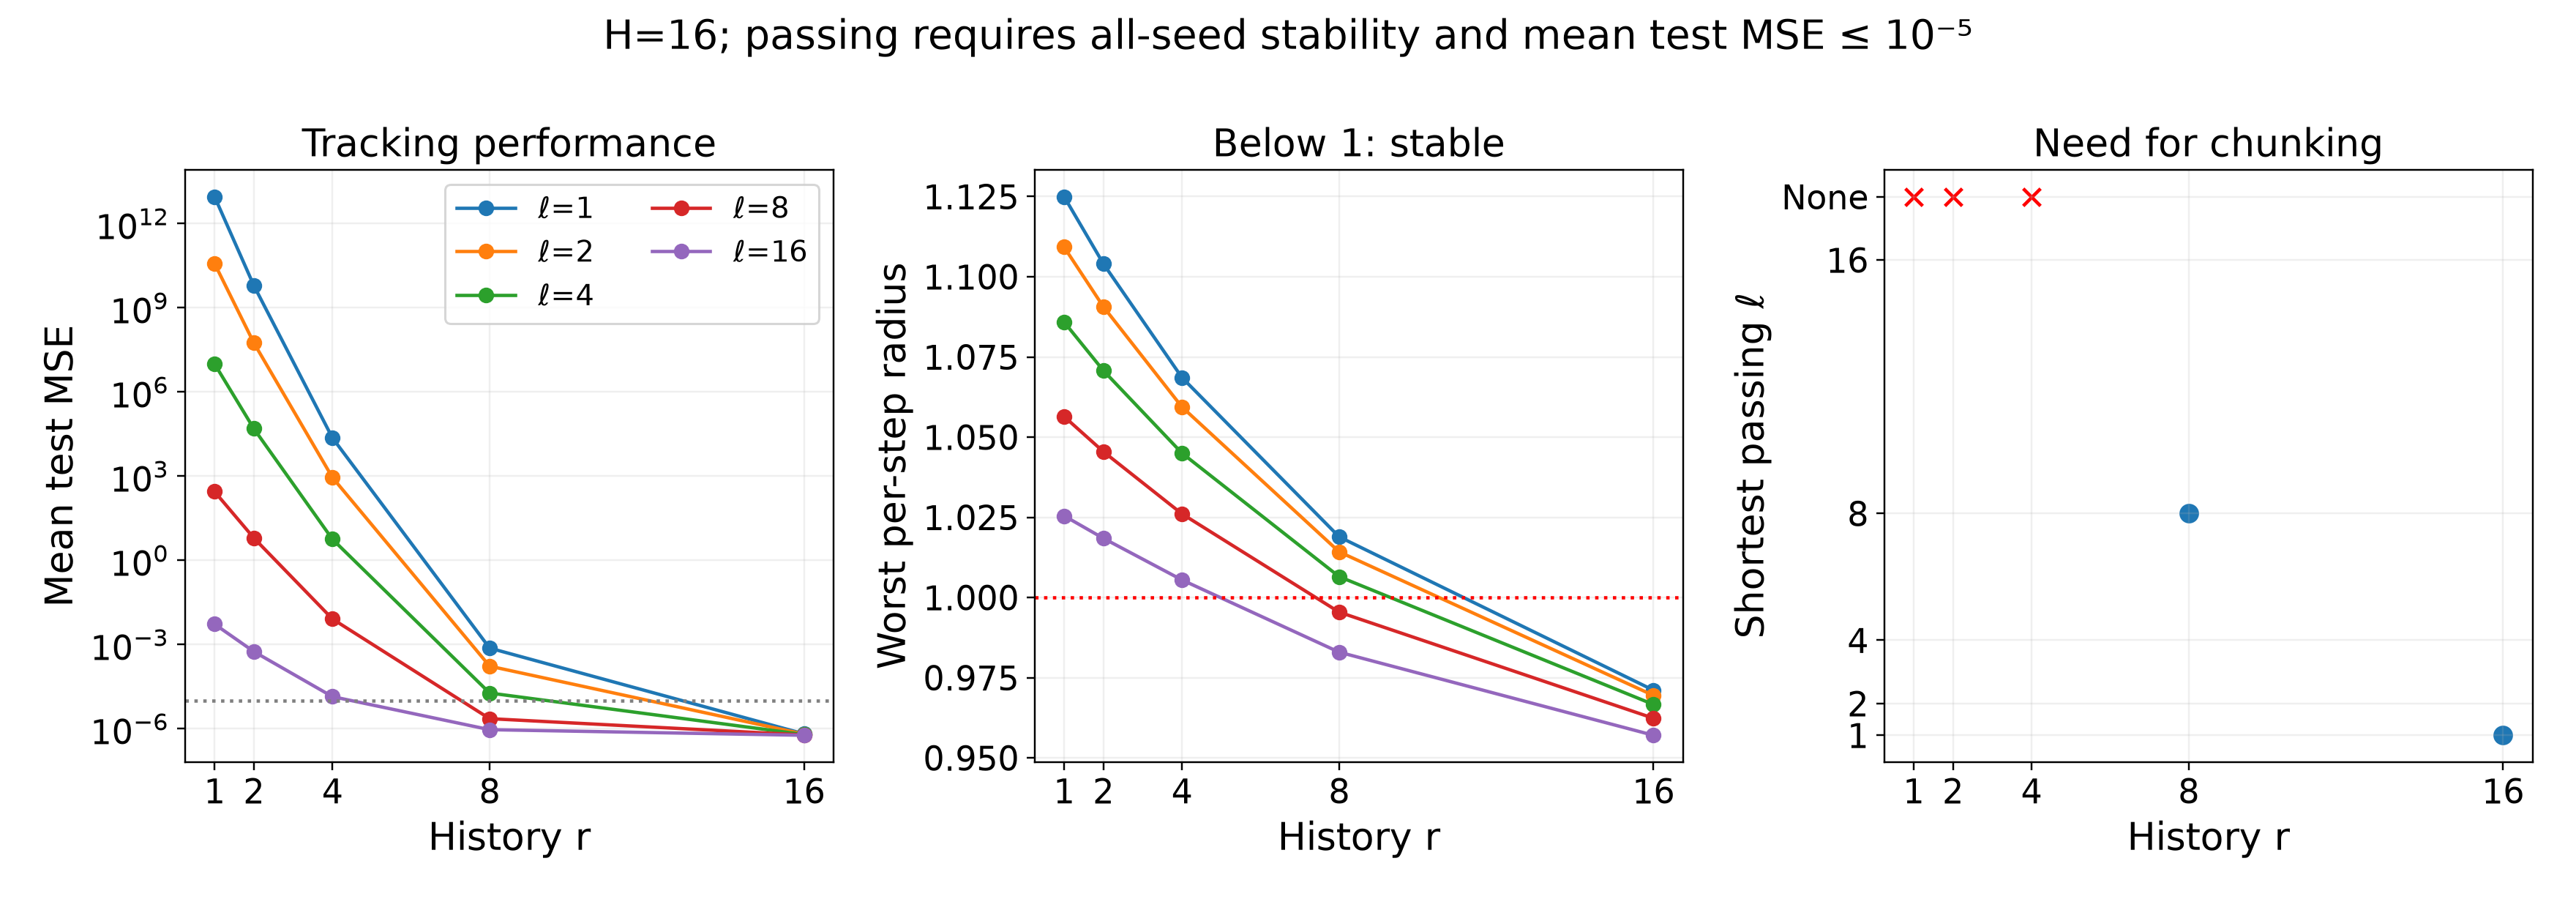
\includegraphics[width=\linewidth]{figures/context_hypothesis.png}
\caption{At $H=16$, history improves test loss and spectral stability. Shortest passing execution is 8 at $r=8$ and 1 at $r=16$; None means no tested setting passes. Passing requires stability and mean test MSE $\le10^{-5}$ for every seed.}
\end{figure}
\vspace{-6pt}
\noindent\textbf{Conclusion.} The current $r=16,\ell=1$ loss is below zero control's $0.08217$, but above the model-informed memory witness's $1.736\times10^{-8}$. Since $h=1$, this is feedback selection rather than hidden-state recovery. The earlier negative narrow-data result used continuing noise and $r\le8$; it is a different protocol. The threshold is illustrative and five seeds give descriptive evidence. Generalizing the tradeoff requires proving that deployment error decreases with context; observability and training fit do not suffice. No result here establishes universal monotonicity of loss.

\begingroup\small
\begin{thebibliography}{2}
\setlength{\itemsep}{0pt}
\bibitem[Simchowitz et al.(2025)]{simchowitz2025}
M. Simchowitz, D. Pfrommer, and A. Jadbabaie.
The pitfalls of imitation learning when actions are continuous.
\emph{arXiv:2503.09722}, 2025.
\bibitem[Zhang et al.(2025)]{zhang2025}
T. T. Zhang, D. Pfrommer, C. Pan, N. Matni, and M. Simchowitz.
Action chunking and exploratory data collection yield exponential improvements in behavior cloning for continuous control.
\emph{arXiv:2507.09061}, 2025.
\end{thebibliography}
\endgroup
\end{document}
